% preamble %
\documentclass[12pt]{article}
\usepackage{amsfonts}
\usepackage{fancyhdr}
\usepackage{comment}
\usepackage[a4paper, top=1cm, bottom=1.5cm, left=2cm, right=2cm]{geometry}
\usepackage{enumitem}
\usepackage{times}
\usepackage{changepage}
\usepackage{amssymb}
\usepackage{graphicx}
\usepackage{tabularx}
\usepackage{titlesec}
\usepackage{hyperref}
\usepackage{changepage}
\usepackage[parfill]{parskip}
\usepackage{wrapfig}
\usepackage[export]{adjustbox}
\usepackage{multirow}
\usepackage{array}
\usepackage[table]{xcolor}

% settings %
\setcounter{secnumdepth}{2} % enumerate
\setcounter{tocdepth}{2}    % TOC entries
\renewcommand{\contentsname}{Innholdsfortegnelse}
\newcounter{fkcounter}
\newcounter{fksubcounter}[fkcounter]
\newcounter{ifkcounter}
\newcounter{ifksubcounter}[ifkcounter]
\titlespacing*{\paragraph}{\parindent}{1ex}{1em}

% commands %
    % counters %
\newcommand*{\FK}{\stepcounter{fkcounter}\textbf{ID: FK\arabic{fkcounter}\\}}
\newcommand*{\FKsub}{\stepcounter{fksubcounter}\textbf{ID: FK\arabic{fkcounter}.\arabic{fksubcounter} \quad}}
\newcommand*{\IFK}{\stepcounter{ifkcounter}\textbf{ID: IFK\arabic{ifkcounter}\\}}
\newcommand*{\IFKsub}{\stepcounter{ifksubcounter}\textbf{ID: FK\arabic{ifkcounter}.\arabic{ifksubcounter} \quad}}
\newcommand{\invis}{\phantom{a}}

    % colors %
\newcommand{\cellr}{\cellcolor{red!25}}
\newcommand{\cello}{\cellcolor{orange!25}}
\newcommand{\celly}{\cellcolor{yellow!25}}
\newcommand{\celll}{\cellcolor{lime!25}}
\newcommand{\cellg}{\cellcolor{green!25}}

% environments %
\newenvironment{subreq}{\begin{adjustwidth}{1cm}{}}{\end{adjustwidth}}

% document %
\begin{document}
\title{%
    Kravspesifikasjon\\
    \large Parkeringsplass reservasjons-app }
\author{Gruppe 12}
\date{}
\maketitle

\newpage

\tableofcontents

\newpage

\section{Problemstilling}

Ofte finner man ikke parkeringsplass mens man er i farta. Det er tett på senterene, gateparkering er privat eller ulovlig og man har ofte dårlig tid. Gjerne etter litt leting finner man en parkering 500 meter unna, og når man kommer dit er det selvfølgelig fullt. Hvordan kan man unngå å miste så mye tid, og i tillegg finne en parkeringsplass?

% Kunden og eksterne partnere kan lese gjennom dokumentasjonen og forstå problemet, hva som skal utvikles og hva som er viktig med systemet som utvikles
\section{Løsningen}
Tjenesten baserer seg på delingsøkonomi og enheten som deles er parkeringsplasser. Ideen er at bedrifter og enkeltpersoner kan registrere en eller flere parkeringsplasser de eier for utleie til enkeltpersoner. Dermed kan disse utleierene tjene penger passivt, samt gjøre det enklere for privatpersoner å forsørge parkering. Parkeringsplassen de legger ut vil være merket med bredde, lengde og høyde, samt om den er reservert for el-biler eller handicappede. På denne måten kan alle som bruker tjenesten få et godt innblikk i parkerings-bildet.

Bruker logger inn som en bedrift eller en vanlig bruker. Brukere kan redigere og legge ut sine registrerte parkeringsplasser, samt leie parkeringsplasser fra andre brukere. Bedrifter kan kun legge ut parkeringsplasser, men har muligheten til å legge til brukere som medlemmer av bedriften. Dette gir de spesialtillatelse til parkeringsplasser som er reservert kun for medlemmer av en spesifikk bedrift. Medlemmer av bedriften vil også kunne legge ut og merke parkeringsplasser for andre bedrifter.

Tjenesten er bygget opp slik at alle brukere har tilgang til en feed som viser en opplisting av de mest relevante parkeringsplassene, en side for registrering av parkeringsplasser og en profilside. For å kunne reservere en parkeringsplass, må bruker oppgi informasjon om bilen de benytter. På feeden rangeres de tilgjengelige parkeringsplassene etter avstand til bruker eller et spesifikt område som bruker spesifiserer, og vises kun dersom de er passende med bilen. Bruker kan også trykke seg inn på et spesifikt innlegg for å se mer detaljer om parkeringsplassen som leies ut, og kan legge en anmeldelse på parkeringsplasser de har brukt. På denne måten får utleiere tilbakemelding på hva de gjør riktig og hva de gjør galt, som bidrar til å øke engasjementet til å gjøre en god jobb.

Kunde av tjenesten vil kunne opprette administratorbrukere som har spesielle egenskaper for administrering av feeden og brukerene. Dette vil være nødvendig for å minke upassende/ulovelig innhold og øke brukeropplevelsen.

\section{Begrensninger og antagelser}


\section{Ansvarsområde og Avhengigheter}
For at man skal kunne kjøre applikasjonen og testene er det noen ting man trenger:


JavaJDK v11
fasterxml.jackson 2.9.9
maven 3.8.0
webjars vue 2.6.10
javalin 3.11.0
JUnit 5.7.0



\section{Funksjoner i applikasjonen}

Programmet henter inn info om brukere, poster, parkeringsplasser og reservasjoner fra en database(i dette tilfellet json-filer). Det programmet gjør nå er å hente inn data fra controller til javalin som generer front-end for oss. Hver side henter da ut nødvendig info hva hver .json fil slik at nødvendig informasjon som adresse og ledighet til leie vises.

Bruker -  Det er mulig å vise oversikt over parkeringsplasser, trykke seg inn til en parkeringsplass, og å legge til en reservasjon, brukeren kan også se oversikt over p-plassene som den har reservert. Det er mulig å legge ut en ny parkeringsplass som en utleier. Det er mulig å vise bilder av parkeringsplassen via et link system, da opplastning direkte til siden ikke er lagt inn. 

Corporation bruker - kan kun legge ut parkeringsplasser. Dette gjør man ved å gå til “My parking spots” hvor “Create new parkingspot” står øverst. For å lage et nytt parkingeringsobjekt må man trykke på denne knappen og fylle ut all nødvendig info(feilmelding dersom ikke alt har noen verdi), og man kan i tillegg velge ved bruk av ikoner dersom det er handikappet eller el-bil plass. Corporation skal kunne få betalt for å leie ut p-plasser.

Admin - Denne brukeren kan suspendere eller slette/banlyse brukere, slette poster og parkeringsplasser. Dette er en bruker-type som i senere iterasjoner kan gi rettigheter til andre brukere (f.eks. modererings-brukere).


\section{Begreper og definisjoner}

\begin{center}
    \begin{tabular}{|p{4cm}|p{12cm}|} 
        \hline
        \bf Begrep & \bf Beskrivelse\\
        \hline
        Applikasjon &  Et programvare som benytter datamaskinens ressurser til en oppgave som brukeren ønsker utført\\
        \hline
        Bruker & Besøkende som samhandler med systemet\\
        \hline
        Brukerkonto & En som kan kun leie parkeringsplasser\\
        \hline
        Bedriftskonto & En som kan kun leie ut parkeringsplasser til andre\\
        \hline
        Administrator & Brukerkonto med administratorrettigheter\\
        \hline
        Feed & Opplisting av innlegg\\
        \hline
        Tjenesten & Tjenesten denne dokumentasjonen omhandler\\
        \hline
        Systemet & Det underliggende systemet til tjenesten\\
        \hline
        Personas & Er et annet ord for rollefigur, enkeltmenneske, karakterpersonlighet\\
        \hline
        ID & Identifikator\\
        \hline
        FK & Funksjonelt Krav (brukes som ID)\\
        \hline
        IFK & Ikke-Funksjonelt Krav (brukes som ID)\\
        \hline
        Innlegg & Brukerinnlegg i systemet (post) som består av en eller flere parkeringsplasser\\
        \hline
        Produktet/ Tjenesten & Applikasjonen som dokumenteres\\
        \hline
        Kunde & Gruppe som eier produktet\\
        \hline
    \end{tabular}
\end{center}

\section{Brukerklasser}
En oversikt over roller og egenskaper for de forskjellige brukerklassene.

    \subsection{Bruker}
    Brukerkontoen er en standardkonto som hvem som helst kan opprette. Som en bruker, kan man registrere sine egne parkeringsplasser og leie andre brukeres parkeringsplasser i perioder. Alle brukere har sin egen profilside der de kan redigere generell informasjon og innstillinger. Brukere kan gi anmeldesler/tilbakemelding på hverandre sine innlegg, og vil bli varslet dersom en annen bruker skriver en anmeldelse på sin parkeringsplass. Ved registrering av parkeringsplass, bestemmer man selv pris og tiden den er tilgjengelig, og den vil automatisk bli vist for andre brukere via feeden eller profil. Man må først registrere bilen man parkerer med før man kan reservere en parkeringsplass.

    \subsection{Bedrift}
    Det er kun organisasjoner som har tilgang til å opprette en bedriftskonto, da de må ha et organisasjonsnummer. Bedriftskontoen er sammensatt av flere brukerkontoer. En brukerkonto som er medlem av en bedrift har spesialtilgang til parkeringsplasser markert for generelle eller spesifikke bedrifter. Bedriftskontoen kan legge ut parkeringsplasser, men kan ikke leie en parkeringsplass. Det er kun bedrifter som kan markere parkeringsplasser for andre bedrifter.

    \subsection{Administrator}
    En administrator ligner en vanligbrukerkonto, men har moen ekstra rettigheter for administraring. De har full makt til å slette brukere, bedrifter, innlegg, parkeringsplasser, og anmeldelser, samt suspendere og oppheve brukerkontoer. Administrator er essensiell for å vedlikeholde en god brukeropplevelse og rettferdiggjøre systemet for alle brukere.

\section{Personaer}

    \subsection{Jørgen Moe}
    
\includegraphics[scale=1]{bilder/personaer/persona_jorgen.jpg}\\
    \textbf{Alder:} 34\\
    \textbf{Jobb/Rolle:}
    Økonom\\
    \textbf{Beskrivelse:}\\
    Jobber som økonom. Han skal grave i gården og lage ny parkeringsplass. Han vet ikke hvor lang tid det kommer til å ta, og han kommer ikke til å ha et sted å parkere i mellomtiden.\\
    \textbf{Motivasjon:}\\
    Han har ikke parkeringsplass hjemme, så han trenger en parkeringsplass i nærheten.\\
    \textbf{Behov:}\\
    Han må kunne forlenge antall dager han låner en parkeringsplass\\
    \textbf{Tekniske ferdigheter:} Gode
    

    \subsection{Siggurd Olson}
    
\includegraphics[scale=1]{bilder/personaer/persona_siggurd.jpg}\\
    \textbf{Alder:} 42\\
    \textbf{Jobb/Rolle:} Ledelse i bedrift\\
    \textbf{Beskrivelse:}\\
    Jobber i ledelsen i en bedrift. Det er ikke alltid han får en plass til å parkere i byen når han skal på jobb.\\
    \textbf{Motivasjon:}\\
    Parkeringsplassene i byen er fullstappa.\\
    \textbf{Behov:}\\
    Han må kunne parkere nærmere arbeidsplassen og sikre seg parkeringplass ved et møte.\\
    \textbf{Tekniske ferdigheter:} Gode

    \subsection{Karina Gausrud}
    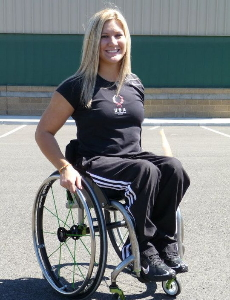
\includegraphics[scale=1]{bilder/personaer/persona_karina.jpg}\\
    \textbf{Alder:} 22\\
    \textbf{Jobb/Rolle:} Uføre\\
    \textbf{Beskrivelse:}\\
    Karina er en rullestolbruker som trenger handicap-parkering. Hun vil helst parkere så nærme målet sitt som mulig, men vet ikke om det finnes en ledig handicap-parkeringsplass. Hun vil heller ikke risikere at stedet ikke tilbyr parkeringsplass for handicappede.\\
    \textbf{Motivasjon:}\\
    Hun trenger en oversikt over ledige handicap-parkeringsplasser.\\
    \textbf{Behov:}\\
    Hun må være sikker på at hun får en handicap-parkeringsplass\\
    \textbf{Tekniske ferdigheter:} Gode

    \subsection{Karin}
    
\includegraphics[scale=1]{bilder/personaer/persona_karin.jpg}\\
    \textbf{Alder:} 34 \\
    \textbf{Jobb/Rolle:} Selger\\
    \textbf{Beskrivelse:}\\
    Karin er dør-til-dør selger, hun kjører til nabolagene hun jobber i hver dag, men det er vanskelig å finne parkering, som gjør at hun taper tid og penger mens hun leter. Derfor åpner hun appen og booker parkeringsplasser for områdene hun skal jobbe den neste måneden. Nå føler Karin at hun har en mindre ting å tenke på.\\
    \textbf{Motivasjon:}\\
    Han har ikke parkeringsplass hjemme, så han trenger en parkeringsplass i nærheten\\
    \textbf{Mål:}\\
    Karin ønsker å eliminere en del av hverdagen som er unødvendig og som koster henne tid og penger. Karin forventer at hun skal finne parkering, og kunne booke det for måneden fremover, eller på dagen om nødvendig.\\
    \textbf{Reisen:}\\
    For å oppnå dette er Karin nødt til å finne utleiere som ønsker kort-tid/dagsutleie, så hun er nødt til å søke området hun skal til, og filtrere til dette alternativet. Deretter kan hun velge sted å parkere basert på beliggenhet og pris i forhold til området hun utvalgte seg.\\
    \textbf{Følelser:}\\
    Karin føler seg frustrert når hun kjører rundt nabolaget hun skal banke dører i, men aldri klarer å finne et sted det er lov å parkere. Karin er på sitt lykkeligste når hun åpner appen for å sjekke hvor hun har bestilt parkering, og vet at hun ikke trenger å tenke på å lete igje\\
    \textbf{Tekniske ferdigheter:} Gode

    \subsection{Jørn Berg}
    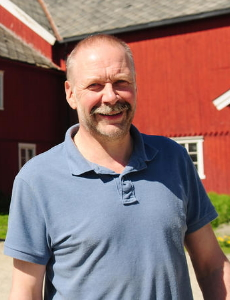
\includegraphics[scale=1]{bilder/personaer/persona_jorn.jpg}\\
    \textbf{Alder:} 56\\
    \textbf{Jobb/Rolle:} Bonde\\
    \textbf{Beskrivelse:}\\
    Jørn bor i nærheten av et vakkert tjern som er populært blant unge å bade i, men siden det ikke er noen parkeringsplass der må folk parkere langs veien. Jørn eier en fin tomt i nærheten der folk kan parkere tryggere.\\
    \textbf{Motivasjon:}\\
    Han vil at tilby parkeringsplasser slik at ungdommene mer sannsynligvis kommer tilbake til tjernet og bader.\\
    \textbf{Behov:}\\
    En omtale system som kan bidra å spre det gode rykte videre. Han vil leie ut tomten for en inntekt ved siden av gårsdriften.\\
    \textbf{Tekniske ferdigheter:} Dårlig

\section{Funksjonelle krav}

    \subsection{Kontoopprettelse}
        
        \subsubsection{Bruker skal kunne opprette en brukerkonto}
        \FK
        For å oppgrette en brukerkonto, må bruker oppgi unikt brukernavn, passord, e-post og telefonnummer.

        \subsubsection{Bruker skal kunne opprette en bedriftskonto}
        \FK
        For å opprette en bedriftskonto, må bruker må oppgi unikt brukernavn, passord, e-post, bedriftsnavn og organisasjonsnummer.

        \subsubsection{Kunden skal kunne opprette brukerkonto med administratorrettigheter}
        \FK
        Kunde har spesialtilgang til å opprette en administrator. 

        \subsubsection{Systemet skal verifisere registreringen}
        \FK
        Systemet må verifisere registreringen via en kode som sjekkes. Denne må bli sendt til brukeren slik at de kan skrive inn koden til programmet. Hvis koden brukeren skriver inn stemmer med den som er lagret i databasen, er registreringen verifisert. Hvis ikke skal de få en feilmelding på samme siden.

            \begin{subreq}
                \FKsub Koden skal være fire-sifret

                \FKsub Bruh 2.1
            \end{subreq}

        \subsubsection{Systemet skal lagre dataen til den brukeren}
        \FK
        Etter at brukeropprettelsen er verifisert, blir data fra opprettelsen lagret i databasen.

        \subsubsection{Derigere opprettet bruker}
        \FK
        Etter opprettelse av konto skal bruker bli ført til startsiden.
    
    \subsection{Innlogging}

        \subsubsection{Bruker skal kunne logge inn som en brukerkonto eller bedriftskonto}
        \FK
        Bruker skal kunne velge å logge inn som en brukerkonto eller bedriftskonto, og så fylle ut tekst-felter med data som stemmer i forhold til opprettelsen av kontoen.

        \subsubsection{Systemet skal verifisere innloggingen}
        \FK
        Dersom innloggingsopplysningene er korrekte i forhold til opplysningene i brukeropprettingen, skal brukeren bli logget inn. Dersom de er ukorrekte, skal brukeren få en feilmeldingen på hva som gikk galt.

        \subsubsection{Derigere innlogget bruker}
        \FK
        Etter vellykket innlogging skal bruker bli ført til startsiden.

    \subsection{Presentasjon av parkeringsplasser (Feed)}

        \subsubsection{Feeden skal vise en liste over relevante parkeringsplasser}
        \FK
        Opplistingen skal bestå av innlegg av parkeringsplasser fra andre brukere.
        
        \subsubsection{Bruker skal kunne sette et filter på feeden}
        \FK
        Opplistingen rangeres via et brukervalgt filter. Filteret bestemmer om opplastingen rangeres basert på nærmest avstand, lavest til høyest pris, høyest til lavest pris, parkeringsplasstype og om den leies ut av en brukerkonto eller bedriftskonto. Standardinnstillingen skal være nærmest avstand.

        \subsubsection{Bruker skal kunne søke etter en adresse}
        \FK
        Feeden skal rangere parkeringsplassene basert på avstand i forhold til denne adressen.

        \subsubsection{Bruker skal kunne søke etter koordinater}
        \FK
        Feeden skal rangere parkeringsplassene basert på avstand i forhold til koordinatene.

    \subsection{Leie parkeringsplass}

        \subsubsection{Bruker skal kunne leie parkeringsplass som en brukerkonto}
        \FK
        Som en brukerkonto skal bruker kunne leie en spesifikk parkeringsplass eller flere parkeringsplasser.

        \subsubsection{Utløp av tid}
        \FK 
        Når en reservert parkeri holder på å gå tom for tid, så skal brukeren som har leid parkeringsplassen få en varsel om at den holder på å gå ut.

    \subsection{Tilbakemelding på innlegg}

        \subsubsection{Bruker skal kunne gi tilbakemelding på et innlegg}
        \FK
        Dersom brukeren har brukt en parkeringsplass, skal de kunne gi tilbakemelding på innlegget til den parkeringsplassen. Innlegget må minst bestå av en poengsum fra 1 til 5, der 5 er den høyeste poengsummen. Om ønskelig kan bruker også legge til en kommentar på maks 130 tegn. Tilbakemeldingen skal lagres i databasen og tilknyttes innlegget.

        \subsubsection{Tilbakemeldinger skal vises på hvert innlegg}
        \FK
        Alle innlegg som tilhører et innlegg skal vises som en liste på innlegget, der nyeste tilbakemelding ligger øverst. Hver tilbakemelding skal vise poengsummen, kommentaren og brukernavn til de som lagde den. I tillegg skal en endelig rangering vises på innlegget som består av gjennomsnittet av poengsummer fra alle tilbakemeldinger knyttet til innlegget.

        \subsubsection{Utleier skal kunne få tilbakemeldinger via mail}
        Ved valg har utleier mulighet til å få alle tilbakemeldinger sendt på mail.

    \subsection{Opprette parkeringsplasser}

        \subsubsection{Bedriftskonto skal kunne registrere en eller flere parkeringsplasser}
        \FK
        For å registrere et parkeringsplass område må de oppgi bredde og lengde i centimeter, antall parkeringsplasser, type parkeringsplass (om det er handikapparkering, eletriskparkering, osv.), etasjer, pris (dette skal kunne endres mauelt eller automastisk i etter kant), postaddresse, gateaddresse og gatenummer.

        \subsubsection{Systemet skal knytte parkeringsplassen til en unik ID}
        \FK
        Den nylig registrerte parkeringsplassen skal knyttes til en unik ID.
        
        \subsubsection{Systemet skal lagre parkeringsplassen i en database}
        \FK
        Den nylig registrerte parkeringsplassen lagres i en database, der den knyttes til en bruker (eier av parkeringsplassen).

    \subsection{Leie betingeleser}

        \subsubsection{Pris}
        \FK
        Eieren av en parkeringsplassen skal kunne justere pris på sin(e) parkeringsplass(er) (i timen).

        \subsubsection{Tid}
        \FK
        Eieren av en parkeringsplassen skal kunne sette en max og min tid for hvor lenge en bil kan stå parkert på en parkeringsplass

        \subsubsection{Regler}
        \FK
        Eieren av en parkeringsplass skal kunne lage sine egne regler for hvordan parkering skal oppholde seg, om det er om tid og/eller kostnad endringer.
        
    \subsection{Betaling}

        \subsubsection{Betale for en parkeringsplass}
        \FK
        Brukeren betaler for parkeringsplassen via valgt betalingsmetode.

        \subsubsection{Tredjepart}
        \FK
        Når en bruker sender inn en forespørsel om å kunne leie en parkeringsplass, så må tredjepart verifisere kjøpet før en bruker kan leie.        

    \subsection{Administrering}

        \subsubsection{Administrator skal kunne bannlyse bruker}
        \FK
        Administrator skal ha full rett til å bannlyse en vilkårlig bruker. Den bannlyste brukeren skal få beskjed om bannlysingen via e-post og direkte i systemet. 

        \subsubsection{Administrator skal kunne slette bruker}
        \FK
        Administrator skal ha full rett til å slette individuelle brukere slik at all tilhørende data blir også slettet fra databasen. Den slettede brukeren skal få beskjed om slettingen via e-post.

        % @TODO: slette?
        % \subsubsection{Administrator skal kunne slette tilbakemeldinger}
        % \FK
        % Administrator skal ha full rett til å slette individuelle tilbakemeldinger på andre innlegg slik at de fjernes både fra grensesnittet og databasen.

        \subsubsection{Administrator skal kunne slette innlegg}
        \FK
        Administrator skal ha full rett til å slette individuelle innlegg. Bruker som lagde innlegget skal få beskjed om slettingen via e-post og direkte i systemet.

        \subsubsection{Administrator skal kunne slette parkeringsplasser}
        \FK
        Administrator skal ha full rett til å slette individuelle parkeringsplasser. Bruker som opprettet parkeringsplassen skal få beskjed om slettingen via e-post og direkte i systemet.

        \subsubsection{Administrator skal kunne slette reservasjoner}
        \FK
        Administrator skal ha full rett til å slette individuelle reservasjoner. Bruker som opprettet reservasjoner skal få beskjed om slettingen via e-post og direkte i systemet.

        \subsubsection{Bedrift skal ha administrerende rettigheter på deres egne innlegg}
        \FK
        Dette innebærer at bedriften kan blokkere brukere av deres egne parkeringsplasser fra å bruke de igjen og slette tilbakemeldinger på deres egne innlegg.

        \subsubsection{Bruker skal kunne rapportere andre brukere sine innlegg}
        \FK
        Brukere har frihet til å rapportere andre brukere sine innlegg. Rapporteringen skal bestå av en begrunnelse. Brukeren som har lagd innlegget skal få varsel via e-post om rapporteringen.

        \subsubsection{Bruker skal kunne rapportere andre brukere}
        \FK
        Brukere har frihet til å rapportere andre brukere. Rapporteringen skal bestå av en begrunnelse. Brukeren som har lagd innlegget skal få varsel via e-post om rapporteringen.
    
    \subsection{Persistent data}

        \subsubsection{Systemet skal lagre informasjon om parkeringsplasser}
        \FK
        Systemet skal lagre all informasjon relatert til enhver parkeringsplass i en tabell i en database eller en lokal fil.

\section{Ikke funksjonelle krav}

    \subsection{Tilgjengelighet}
    \IFK
    All brukere skal ha tilgang til applikasjonen til enhver tid.
    
    \subsection{Sikkerhetskopi(Backup)}
    \IFK
    Sikkerhetskopiering av database skal skje hver 24 time kl 04.00

    \subsection{Dependency på tredjepart}
    \IFK
    Betaling verifiseres og håndteres av NETS

    \subsection{Legal and licensing issues}


    \subsection{Nettverkstopologi}


    \subsection{Preformance / response time}


    \subsection{Personvern}


    \subsection{Kvalitet}


    \subsection{Sikkerhet}


    \subsection{Supportability}


    \subsection{Testability}
        
    \subsection{Interface}

% @TODO: Fremtidig implementasjon
%
% \subsubsection{Bruker kan ha flere biler}
% Når en kunde skal resevere en parkeringsplass, så kan det hende at de har tilgang på flere biler og de skal de bilen være lagret etter bruk i brukerns database.
%
% \subsubsection{Lagre/Favorit}
% En kunde kan bruke den samme parkeringsplassen flere ganger og vil sikkert ha en kjapp måtte å koble seg opp mot den bestemte parkeringsplassen.

\section{Prototype}

    \subsection{Sammendrag}

    \subsection{Innstallasjon}
    For å bygge og kjøre programmet åpner man hele mappen som et intellij prosjekt, da vil også alle avhengigheter bli installert, eller det vil komme en installasjonsprompt med beskrivelse i terminalen i  intelliJ(dette skjer for npm installasjon). Dersom dette skjer fullfører du installasjonen som beskrives i terminalen. Deretter må man trykke på den grønne hammeren i høyere hjørnet eller ctrl+f9 for å bygge programmet.

    \subsection{Bruksmanual}
    For å starte programmet velger man main metoden i drop-down menyen og trykker grønn pil eller shitf+f10. Da vil javalin kjøre i konsollen i intellij, og det vil åpne seg port på http://localhost:7000/ . Når man trykker på den kommer man en hovedside med tre knapper. En for bruker, en for corporation og en for admin.
    
    Når man har kommet inn til localhost:7000 blir man presentert med tre knapper. En for bruker, en for corporation og en for admin. Bruker knappen leder til parkeringsplass oversikten der alle tilgjengelige plasser vises. Derfra kan bruker trykke seg inn på en parkeringsplass, trykke seg inn til bestillings-siden, og fylle ut ordren, og trykke submit knappen for å bestille, da skal den dukke opp i “My parking spots” på bunnen av siden der det står reservasjoner.
    
    Inne på denne siden kan brukeren opprette parkeringsplasser de ønsker å leie ut ved å trykke på “Create new parking spot”-knappen der de taes til en skjema for utfylling. Dersom skjema ikke er tilstrekkelig utfylt vil en feilmelding vises med all info som er nødvendig i skjemaet. Når skjema er riktig utfylt kan man trykke submit knappen, og den nye parkeringsplassen vil umiddelbart være postet til både hovedoversikten og til brukerens “My parking spots”-side. Foreløpig fungerer corporation-brukeren på lik linje som bruker-typen.
    
    Da man trykker admin-typen kommer man til en oversikt over brukere, parkeringsplasser, poster og reservasjoner. Admin kan suspendere eller slette kontoer, og den kan slette parkeringsplasser, poster og reservasjoner.

    \subsection{Implementerte krav og tester}
    For å kjøre backend testene må man åpne test-mappen i intelliJ og høyre-klikke på den grønne java-mappen, og velge Run ‘All Tests’ With Coverage. Da kjører man testene og kan se andelen av programmet der det er test-dekning.

    \subsection{Avhengigheter}

    \subsection{Begrensninger}

\section{Diagrammer}
    \subsection{Sekvesndiagram - Leie en parkeringplass.}
    \includegraphics[max width=\textwidth]{bilder/diagrammer/Sekvensdiagram-LeieEnParkeringsplass-Håkon.png}

    \subsection{Dataflytdiagram - Tilbakemelding}
    \includegraphics[max width=\textwidth]{bilder/diagrammer/Dataflytdiagram-TilbakemeldingOgPoengsum-Håkon.png}

    \subsection{Sekvensdiagram - Opprette reservasjon}
    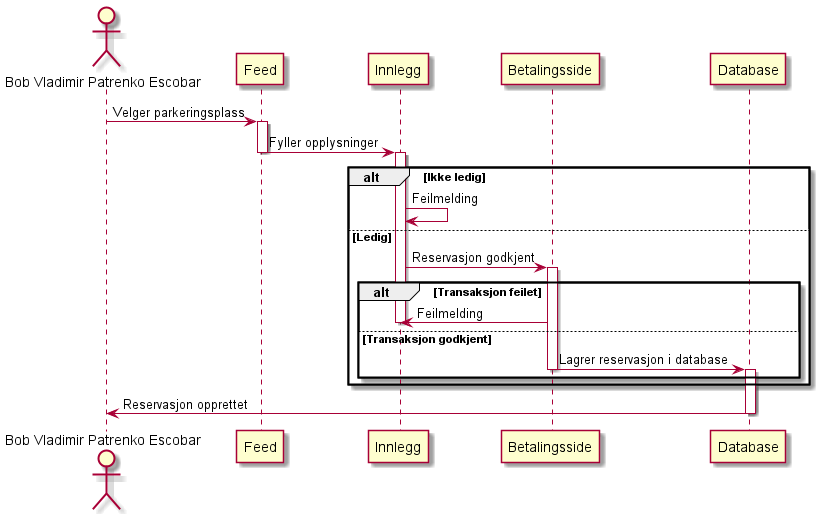
\includegraphics[max width=\textwidth]{bilder/diagrammer/opprette reservasjon_sekvensdiagram.png}

    \subsection{Tilstandsdiagram - Registrere parkeringsplass}
    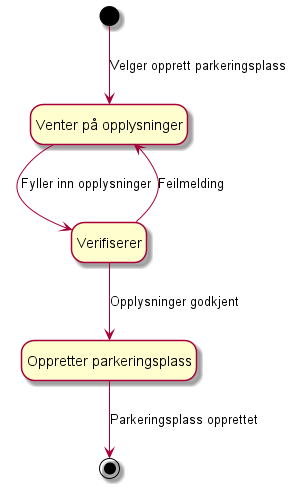
\includegraphics[max width=\textwidth]{bilder/diagrammer/opprett_parkeringsplass_tilstandsdiagram.png}
    
        \subsubsection{Forklaring}
        Når bruker oppretter parkeringsplass venter systemet på en POST forespørsel med informasjon om gatenavn, adresse, bredde, lengde og høyde, samt informasjon angående parkeringsplasstype (handicap, el-bil, osv.). Dersom opplysningene ikke tilfredstiller forventningene i systemet, får bruker en feilmelding og blir nødt til å fylle ut på nytt. Dersom opplysningene er godkjent blir parkeringsplassen opprettet. 

    \subsection{Aktivitetsdiagram - Leie en parkeringsplass}
    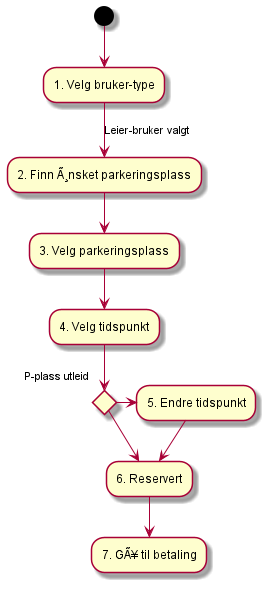
\includegraphics[max width=\textwidth]{bilder/diagrammer/leierAktivitetBestilling.png}

    \subsection{Sekvensdiagram - Leie ut en parkeringsplass}
    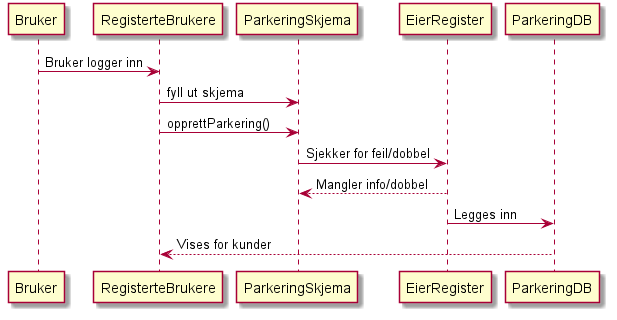
\includegraphics[max width=\textwidth]{bilder/diagrammer/sekvensdiagramLeggeUtParkering.png}

\section{Estemering}

    \subsection{Enheter}

    \begin{tabular}{|p{2cm}|
        >{\centering\arraybackslash}p{3cm}|
        >{\centering\arraybackslash}p{3cm}|
        >{\centering\arraybackslash}p{3cm}|
        >{\centering\arraybackslash}p{3cm}|}     
        \hline 
        \invis & \multicolumn{4}{|c|}{Utviklingsstørrelse}\\
        \hline
        Verdi & X-Large & Large & Medium & Small\\
        \hline
        X-Large &   \celly0 &
                    \cellg4 &
                    \cellg6 &
                    \cellg7 \\
        \hline
        Large &     \cellr-4 &
                    \celly0 &
                    \celll2 &
                    \cellg3 \\
        \hline
        Medium &    \cellr-6 &
                    \cello-2 &
                    \celly0 &
                    \celll1 \\
        \hline
        Small &     \cellr-7 &
                    \cellr-3 &
                    \cello-1 &
                    \celly0 \\
        \hline 
    \end{tabular}

    \subsection{Estimeringstabell - Funksjonelle krav}
        \begin{tabular}{|p{2cm}|p{4cm}|p{4cm}|p{4cm}| } 
            \hline
            \bf EsID & \bf Vikitighet & \bf Vanskelighetsgrad & \bf Utviklingsstørrelse\\
            \hline
            FK1 & NULL & NULL & NULL\\
            \hline
            FK2 & NULL & NULL & NULL\\
            \hline
            FK3 & NULL & NULL & NULL\\
            \hline
            FK4 & NULL & NULL & NULL\\
            \hline
            FK5 & NULL & NULL & NULL\\
            \hline
            FK6 & NULL & NULL & NULL\\
            \hline
            FK7 & NULL & NULL & NULL\\
            \hline
            FK8 & NULL & NULL & NULL\\
            \hline
            FK9 & NULL & NULL & NULL\\
            \hline
            FK10 & NULL & NULL & NULL\\
            \hline
            FK11 & NULL & NULL & NULL\\
            \hline
            FK12 & NULL & NULL & NULL\\
            \hline
            FK13 & NULL & NULL & NULL\\
            \hline
            FK14 & NULL & NULL & NULL\\
            \hline
            FK15 & NULL & NULL & NULL\\
            \hline
            FK16 & NULL & NULL & NULL\\
            \hline
            FK17 & NULL & NULL & NULL\\
            \hline
            FK18 & NULL & NULL & NULL\\
            \hline
            FK19 & NULL & NULL & NULL\\
            \hline
            FK20 & NULL & NULL & NULL\\
            \hline
            FK21 & NULL & NULL & NULL\\
            \hline
            FK22 & NULL & NULL & NULL\\
            \hline
            FK23 & NULL & NULL & NULL\\
            \hline
            FK24 & NULL & NULL & NULL\\
            \hline
            FK25 & NULL & NULL & NULL\\
            \hline
            FK26 & NULL & NULL & NULL\\
            \hline
            FK27 & NULL & NULL & NULL\\
            \hline
            FK28 & NULL & NULL & NULL\\
            \hline
            FK29 & NULL & NULL & NULL\\
            \hline
            FK30 & NULL & NULL & NULL\\
            \hline
            FK31 & NULL & NULL & NULL\\
            \hline
            FK32 & NULL & NULL & NULL\\
            \hline
            FK33 & NULL & NULL & NULL\\
            \hline
            FK34 & NULL & NULL & NULL\\
            \hline
            FK35 & NULL & NULL & NULL\\
            \hline
            FK36 & NULL & NULL & NULL\\
            \hline
        \end{tabular}

    \subsection{Estimeringstabell - Ikke funksjonelle krav}
        \begin{tabular}{|p{2cm}|p{4cm}|p{4cm}|p{4cm}| } 
            \hline
            \bf EsID & \bf Vikitighet & \bf Vanskelighetsgrad & \bf Utviklingsstørrelse\\
            \hline
            IFK1 & NULL & NULL & NULL\\
            \hline
        \end{tabular}


\end{document}